

\subsection{MIT-Access Card}

MIT card inculde both a magnetic strip and an RFID tag (125 kHz).
An analysis showed that eavesdropping twice the communication 
reveals the same broadcast.
\begin{itemize}
    \item Broadcast contains 224 bits with only 32 bits \textbf{change}
            from card to card
    \item[$\Rightarrow$]An attack can be done by replaying a recording
        of a previously broadcasted value.
\end{itemize}

The card uses low frequency $\Rightarrow$ easy to listen/emit by an adversary. Also the card only broadcasts an UID $\Rightarrow$ Replay attack.

\subsection{EMV-CAP}

Used by bank to authenticate customers online 
\begin{itemize}
	\item Mode 1 : Authentication to get access to an e-banking account 
	\begin{center}
		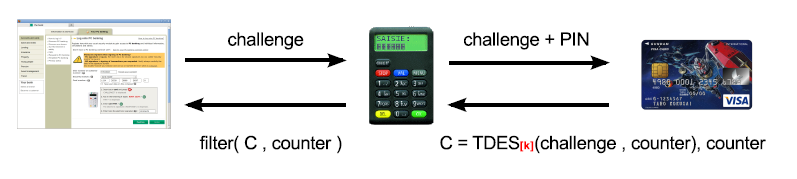
\includegraphics[scale=0.6]{img/mode1-ebanking}
	\end{center}
	
	\item Mode 2 : Signature of a financial transaction
	\begin{center}
		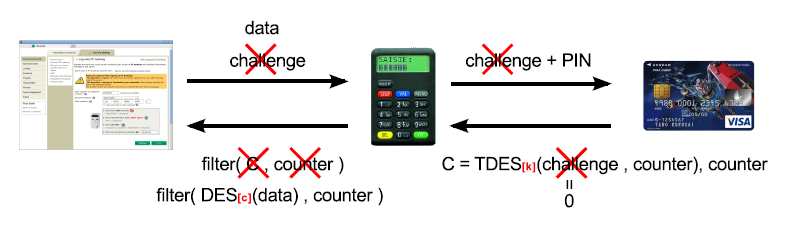
\includegraphics[scale=0.6]{img/mode2-ebanking}
	\end{center}
\end{itemize}
The first mode is secure but with the second replay attack is possible. %preplay too?


\subsection{Digital Signature Transponder}


Texas Instruments Digital Signature Transponder is a tag used to enable 
fuel-injection system of the vehicle.
\begin{itemize}
	\item It uses a Proprietary cipher that uses 40-bit keys
	\item DST responses to 8 queries per second.
\end{itemize}

\subsubsection{Authentication protocol}
\begin{tabular}{m{8cm}m{8cm}}
    \begin{tabular}{ccc}
        Verifier & & Prover \\
                 &\fr{r} & \\
        \\
        & \fl{id, $Trunc_{24}(E_k(r))$, checksum} \\
    \end{tabular}
    &
    \begin{itemize}
        \item |k| = |r| = |$E_k(r)$| = 40bits
        \item |identifier| = |$Truncate_{24}(E_k(r))$| = 24 bits
        \item |checksum| = 16 bits
    \end{itemize}
\end{tabular}

\subsubsection{Attacks}
%TODO understand weakness
An attack has been performed on this system which consist of:
\begin{enumerate}
	\item Reverse engineering the cipher
	\item Eavesdropping some communications\footnote{One communication is
    sufficient if no truncation as the truncation is a mapping N to 1}
	\item Recovering the key using a brute force attack (feasible as $|k|$ is small)
	\item Simulating the tag to ignit the targeted tag
\end{enumerate}
\paragraph{Security}
\begin{itemize}
	\item Because the tag respond to any challenge, it's possible to challenge it instead
	of eavesdropping it
	\item Since the tag response is truncated, using a brute force on one 
	challenge/response pair leads to several possible keys ( pigeonhole principle)
	\item Authors managed to recover a key with 16 FGPAs in parallel
\end{itemize}
